
\subsection{Transition systems}
\label{sec:ts}

\begin{definition}[TS on graphs]
  A transition system on graphs $TS = (Q,R,T)$ consists of
  \begin{itemize}
  \item a set of states $Q\subseteq \mathcal{G}$, where each state is a simple graph;
  \item a set of rules or productions, $R$;
  \item a set of labelled transition $T\subseteq Q\times \text{hom}(\mathcal{G})\times R\times Q$, where each transition $M \overset{m,p}{\Rightarrow} N$ is a dpo rewriting step with the production $p\in R$, $p:L\lemb K\remb R$ and the matching $m:L\emb M$.
  \end{itemize}
\end{definition}

%We denote $t:(s,e,s')$ a transition.
Transitions can be composed $t_1;t_2$ if the source state of $t_2$ matches the destination state of $t_1$. A \emph{trace} $\theta$ is a sequence of composable transitions: $\theta=t_1;t_2;\cdots t_n$. Two traces $\theta:t_1;\cdots t_n$ and $\theta':t_1';\cdots t_n'$ can be composed if $t_n$ and $t_1'$ are composable: $\theta;\theta':t_1;\cdots t_n;t_1;\cdots t_n'$.

\begin{definition}[Independence relation on transitions~\cite{AlgebraicGR}]
  \label{def:indep}
  $~$
  \begin{description}
  \item[sequential independence]
    Let $t_1:M\overset{m_1,p_1}{\Rightarrow} M_1$ and $t_2:M_1\overset{m_2,p_2}{\Rightarrow} M_2$ be two transitions.
    $t_1 \Diamond_{\text{seq}} t_2$ iff there exists the morphism $i:R_1\emb D_2$ such that $i\circ f_2 = n_1$ and there exists the morphism $j:L_2\emb D_1$ such that $j\circ g_1= m_2$:
    \[
    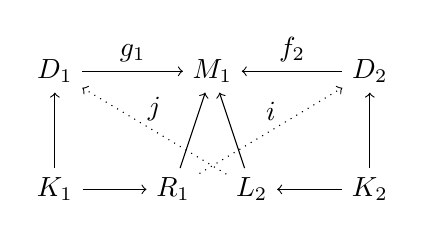
\begin{tikzpicture} %[scale=0.8]
    \node (r1) at (1.5,0) {\(R_1\)};
    \node (m1) at (2,1.5) {\(M_1\)};
    \node (l2) at (2.5,0) {\(L_2\)};
    \node (d1) at (0,1.5) {\(D_1\)};
    \node (k1) at (0,0) {\(K_1\)};
    \node (d2) at (4,1.5) {\(D_2\)};
    \node (k2) at (4,0) {\(K_2\)};
    \draw [->] (k1) -- (r1);
    \draw [->] (k2) -- (l2);
    \draw [->] (k1) -- (d1);
    \draw [->] (k2) -- (d2);
    \draw [->] (d1) -- node [above,midway] {\(g_1\)} (m1);
    \draw [->] (d2) -- node [above,midway] {\(f_2\)} (m1);
    \draw [->] (l2) -- (m1);
    \draw [->] (r1) -- (m1);
    \draw [dotted,->] (r1) -- node [above,midway] {\(i\)} (d2);
    \draw [dotted,->] (l2) -- node [above,midway] {\(j\)} (d1);
    \end{tikzpicture}
    \]
  \item[parallel independence]
    Let $t_1:M\overset{m_1,p_1}{\Rightarrow} M_1$ and $t_2:M\overset{m_2,p_2}{\Rightarrow} M_2$ be two transitions.
    $t_1 \Diamond_{\text{par}} t_2$ iff there exists the morphism $i:L_1\emb D_2$ such that $i\circ f_2= n_1$ and there exists the morphism $j:L_2\emb D_1$ such that $j\circ f_1= m_2$:
    \[
    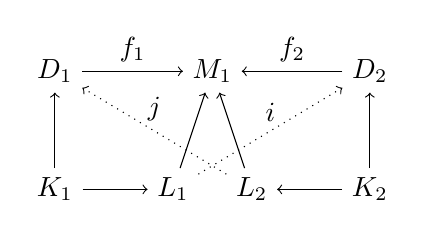
\begin{tikzpicture} %[scale=0.8]
    \node (r1) at (1.5,0) {\(L_1\)};
    \node (m1) at (2,1.5) {\(M_1\)};
    \node (l2) at (2.5,0) {\(L_2\)};
    \node (d1) at (0,1.5) {\(D_1\)};
    \node (k1) at (0,0) {\(K_1\)};
    \node (d2) at (4,1.5) {\(D_2\)};
    \node (k2) at (4,0) {\(K_2\)};
    \draw [->] (k1) -- (r1);
    \draw [->] (k2) -- (l2);
    \draw [->] (k1) -- (d1);
    \draw [->] (k2) -- (d2);
    \draw [->] (d1) -- node [above,midway] {\(f_1\)} (m1);
    \draw [->] (d2) -- node [above,midway] {\(f_2\)} (m1);
    \draw [->] (l2) -- (m1);
    \draw [->] (r1) -- (m1);
    \draw [dotted,->] (r1) -- node [above,midway] {\(i\)} (d2);
    \draw [dotted,->] (l2) -- node [above,midway] {\(j\)} (d1);
    \end{tikzpicture}
    \]
  \end{description}
\end{definition}

\begin{lemma}[Local Church Rosser Theorem~\cite{AlgebraicGR}]
  \label{church_rosser}
  If two transitions $t_1:M\overset{m_1,p_1}{\Rightarrow} M_1$ and $t_2:M_1\overset{m_2,p_2}{\Rightarrow} M_2$ are sequentially independent, there exists $M'\in Q$ and two transitions $t_2':M\overset{m_2',p_2}{\Rightarrow} M'$ and $t_1':M'\overset{m_1',p_1}{\Rightarrow} M_2$. Moreover, $t_1$ and $t_2'$ are parallel independent.

If two transitions $t_1:M\overset{m_1,p_1}{\Rightarrow} M_1$ and $t_2:M\overset{m_2,p_2}{\Rightarrow} M_2$ are parallel independent, then there exists $M'\in Q$ and two transitions $t_2':M_1\overset{m_2',p_2}{\Rightarrow} M'$ and $t_1':M_2\overset{m_1',p_1}{\Rightarrow} M'$. Moreover, $t_1$ and $t_2'$ (and $t_2$, $t_1'$) are sequential independent.
\end{lemma}


\begin{definition}[Dependence relation on transitions]
  \label{def:dep}
  Let $t_1:M_1\overset{m_1,p_1}{\Rightarrow} N_1$ and $t_2:M_2\overset{m_2,p_2}{\Rightarrow} N_2$ be two transitions in a trace $\theta:t_1;t_1':t_2';\cdots t_n';t_2$ and let $p_1:L_1{\remb} D_1 {\lemb} R_1$ and $p_2:L_2{\remb} D_2 {\lemb} R_2$ be two corresponding rules. The morphism $N_1\pmorph M_2$ is the composition of $\spo(t_1')\circ\dots\spo(t_n')$.
  \begin{description}
%  \item[] $~$
  \item[high res dependence]
    Let the span $\spa:R_1\remb O\lemb L_2$ be the pullback of the cospan $R_1{\lemb}M{\remb}L_2$ in the multisum of $R_1$ and $L_2$ such that $p_1\redl{+}_{\spa} p_2$. If the diagram commutes
  \[
  \begin{tikzpicture} %[scale=0.8]
    \node (o) at (1,0) {\(O\)};
    \node (m) at (1,2) {\(M\)};
    \node (m1) at (-2,3) {\(M_1\)};
    \node (n1) at (0,3) {\(N_1\)};
    \node (n2) at (4,3) {\(N_2\)};
    \node (m2) at (2,3) {\(M_2\)};
    \node (r1) at (0,1) {\(R_1\)};
    \node (l1) at (-2,1) {\(L_1\)};
    \node (l2) at (2,1) {\(L_2\)};
    \node (r2) at (4,1) {\(R_2\)};
    \draw [->] (o) -- (r1);
    \draw [->] (o) -- (l2);
    \draw [->] (r1) --  (m);
    \draw [->] (r1) --  (n1);
    \draw [->] (l2) --  (m);
    \draw [->] (l2) --  (m2);
    \draw [->] (m) --  (n1);
    \draw [->] (m) --  (m2);
    \draw [-{Stealth[left]}] (n1) --  (m2);
    \draw [->] (l1) --  (m1);
    \draw [->] (r2) --  (n2);
    \draw [vecArrow] (m1) -- node [above,midway] {$m_1,p_1$} (n1);
    \draw [vecArrow] (m2) -- node [above,midway] {$m_2,p_2$} (n2);
    \draw [vecArrow] (l2) -- (r2);
    \draw [vecArrow] (l1) -- (r1);
  \end{tikzpicture}
  \]
  then $t_2$ is high res dependent on $t_1$, denoted $t_1 < t_2$.
\item[low res dependence]
%  Let $t_1:M_1\overset{m_1,p_1}{\Rightarrow} N_1$ and $t_2:M_2\overset{m_2,p_2}{\Rightarrow} N_2$ be two transitions and let $p_1:L_1{\remb} D_1 {\lemb} R_1$ and $p_2:L_2{\remb} D_2 {\lemb} R_2$ be two corresponding rules.
If there exists $\spa:R_1\remb O\lemb L_2$ such that $p_1\redl{+}_{\spa} p_2$ and such that the diagram commutes
  \[
  \begin{tikzpicture} %[scale=0.8]
    \node (o) at (1,0) {\(O\)};
    \node (m1) at (-2,3) {\(M_1\)};
    \node (n1) at (0,3) {\(N_1\)};
    \node (n2) at (4,3) {\(N_2\)};
    \node (m2) at (2,3) {\(M_2\)};
    \node (r1) at (0,1) {\(R_1\)};
    \node (l1) at (-2,1) {\(L_1\)};
    \node (l2) at (2,1) {\(L_2\)};
    \node (r2) at (4,1) {\(R_2\)};
    \draw [->] (o) -- (r1);
    \draw [->] (o) -- (l2);
    \draw [->] (r1) --  (n1);
    \draw [->] (l2) --  (m2);
    \draw [-{Stealth[left]}] (n1) --  (m2);
    \draw [->] (l1) --  (m1);
    \draw [->] (r2) --  (n2);
    \draw [vecArrow] (m1) -- node [above,midway] {$m_1,p_1$} (n1);
    \draw [vecArrow] (m2) -- node [above,midway] {$m_2,p_2$} (n2);
    \draw [vecArrow] (l2) -- (r2);
    \draw [vecArrow] (l1) -- (r1);
  \end{tikzpicture}
  \]
  then $t_2$ is low res dependent on $t_1$, denoted $t_1 \prec t_2$.
  \end{description}
\end{definition}
Note that $t_1< t_2 \implies t_1\prec t_2$ but not the reverse.

\begin{definition}[Inhibition relations on transitions]
  \label{def:inhibition}
  Let $t_1:M_1\overset{m_1,p_1}{\Rightarrow} N_1$ and $t_2:M_2\overset{m_2,p_2}{\Rightarrow} N_2$ be two transitions in a trace $\theta:t_1;t_1':t_2';\cdots t_n';t_2$ and let $p_1:L_1{\remb} D_1 {\lemb} R_1$ and $p_2:L_2{\remb} D_2 {\lemb} R_2$ be two corresponding rules. The morphism $M_1\pmorph M_2$ is the composition of $\spo(t_1)\circ\spo(t_1')\circ\dots\spo(t_n')$.
  \begin{description}
  \item[high res inhibition]
    Let the span $\spa:L_1\remb O\lemb L_2$ be the pullback of the cospan $L_1{\lemb}M{\remb}L_2$ in the multisum of $L_1$ and $L_2$ such that $p_1\redl{-}_{\spa} p_2$. If the diagram commutes
  \[
  \begin{tikzpicture} %[scale=0.8]
    \node (o) at (1,0) {\(O\)};
    \node (m) at (1,2) {\(M\)};
    \node (m1) at (0,3) {\(M_1\)};
    \node (n2) at (4,3) {\(N_2\)};
    \node (m2) at (2,3) {\(M_2\)};
    \node (l1) at (0,1) {\(L_1\)};
    \node (l2) at (2,1) {\(L_2\)};
    \node (r2) at (4,1) {\(R_2\)};
    \draw [->] (o) -- (l1);
    \draw [->] (o) -- (l2);
    \draw [->] (l1) --  (m);
    \draw [->] (l1) --  (m1);
    \draw [->] (l2) --  (m);
    \draw [->] (l2) --  (m2);
    \draw [->] (m) --  (m1);
    \draw [->] (m) --  (m2);
    \draw [-{Stealth[left]}] (m1) --  (m2);
    \draw [->] (r2) --  (n2);
    \draw [vecArrow] (m2) -- node [above,midway] {$m_2,p_2$} (n2);
    \draw [vecArrow] (l2) -- (r2);
  \end{tikzpicture}
  \]
  then $t_2$ is high res inhibiting $t_1$, denoted $t_2 \Dashv t_1$.
\item[low res inhibition]
  If there exists $\spa:L_1\remb O\lemb L_2$ such that $p_1\redl{-}_{\spa} p_2$ and such that the diagram commutes
  \[
  \begin{tikzpicture} %[scale=0.8]
    \node (o) at (1,0) {\(O\)};
    \node (m1) at (0,3) {\(M_1\)};
    \node (n2) at (4,3) {\(N_2\)};
    \node (m2) at (2,3) {\(M_2\)};
    \node (l1) at (0,1) {\(L_1\)};
    \node (l2) at (2,1) {\(L_2\)};
    \node (r2) at (4,1) {\(R_2\)};
    \draw [->] (o) -- (l1);
    \draw [->] (o) -- (l2);
    \draw [->] (l1) --  (m1);
    \draw [->] (l2) --  (m2);
    \draw [-{Stealth[left]}] (m1) --  (m2);
    \draw [->] (r2) --  (n2);
    \draw [vecArrow] (m2) -- node [above,midway] {$m_2,p_2$} (n2);
    \draw [vecArrow] (l2) -- (r2);
  \end{tikzpicture}
  \]
  then $t_2$ is low res inhibiting $t_1$, denoted $t_1 \dashv t_2$.
  \end{description}
\end{definition}
Note that $t_1\Dashv t_2 \implies t_1\dashv t_2$ but not the reverse.

When we want to make the underlying span explict, we write $t_1 <^{\spa} t_2$, $t_1 \prec^{\spa} t_2$, $t_1 \dashv^{\spa} t_2$ and $t_1 \Dashv^{\spa} t_2$, respectively.

\begin{example}
  For a trace $t_1;t_2;t_3$ with the transitions
  \[
  t_1: A \Rightarrow A,B\qquad t_2: A,B\Rightarrow B,C \qquad t_3: B,C\Rightarrow D
  \]
  one can deduce $t_1\prec t_2$ but cannot deduce $t_1<t_3$, as transitions $t_1$ and $t_2$ do not commute.
\end{example}

\begin{lemma}
  \label{lem:seq_dep}
  Two sequential transitions $t_1:M\overset{m_1,p_1}{\Rightarrow} M_1$ and $t_2:M_1\overset{m_2,p_2}{\Rightarrow} M_2$ are high res dependent if and only if there exists no morphism $j:L_2\emb D_1$ such that $j\circ g_1= m_2$.
\end{lemma}
\begin{proof}
  First note that for any injective morphism in the diagram we can define a bijection between the domain and the image of the morphism in the codomain. Secondly note that for any graph $M_1$ there exists a unique $M$ in the multisum of $R_1$ and $L_2$ that commutes:
  \[
  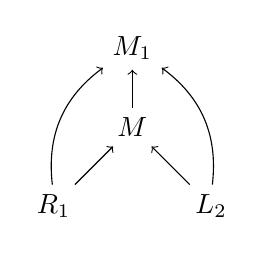
\begin{tikzpicture} %[scale=0.8]
    \node (r1) at (1,0) {\(R_1\)};
    \node (m1) at (2,2) {\(M_1\)};
    \node (m) at (2,1) {\(M\)};
    \node (l2) at (3,0) {\(L_2\)};
    \draw [->] (r1) -- (m);
    \draw [->] (l2) -- (m);
    \draw [->] (m) -- (m1);
    \draw [->] (r1) to [bend left] (m1);
    \draw [->] (l2) to [bend right] (m1);
    \end{tikzpicture}
    \]
    and that the pullback of $R_1\lemb M_1\remb L_2$ is the same as the pullback of $R_1\lemb M\remb L_2$. Therefore we can reason using the span $R_1\lemb M_1\remb L_2$ in what follows.

    Let $R_1\remb O \lemb L_2$ be the pullback of the cospan $R_1\lemb M_1\remb L_2$ and let $K_1\remb P \lemb O$ be the pullback of $K_1\lemb R_1\remb O$.
  We proceed by showing that in the diagram below
    \[
    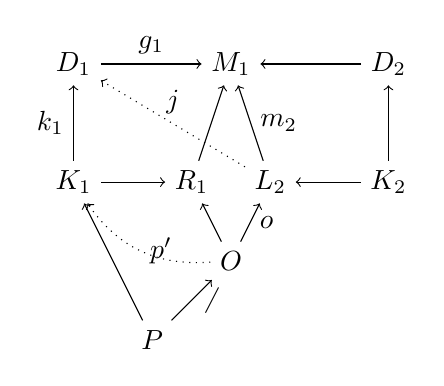
\begin{tikzpicture} %[scale=0.8]
    \node (r1) at (1.5,0) {\(R_1\)};
    \node (m1) at (2,1.5) {\(M_1\)};
    \node (l2) at (2.5,0) {\(L_2\)};
    \node (d1) at (0,1.5) {\(D_1\)};
    \node (k1) at (0,0) {\(K_1\)};
    \node (d2) at (4,1.5) {\(D_2\)};
    \node (k2) at (4,0) {\(K_2\)};
    \node (o) at (2,-1) {\(O\)};
    \node (p) at (1,-2) {\(P\)};
    \draw [->] (k1) -- (r1);
    \draw [->] (k2) -- (l2);
    \draw [->] (k1) -- node [left,midway] {\(k_1\)} (d1);
    \draw [->] (k2) -- (d2);
    \draw [->] (d1) -- node [above,midway] {\(g_1\)} (m1);
    \draw [->] (d2) -- (m1);
    \draw [->] (l2) -- node [right,midway] {\(m_2\)} (m1);
    \draw [->] (r1) -- (m1);
    \draw [dotted,->] (l2) -- node [above,midway] {\(j\)} (d1);
    \draw [->] (p) -- (k1);
    \draw [->] (p) -- node [right,midway] {$\not\iso$} (o);
    \draw [->] (o) -- (r1);
    \draw [->] (o) -- node [right,midway] {$o$} (l2);
    \draw [dotted,->] (o) to [bend left] node [right,midway] {$p'$} (k1);
    \end{tikzpicture}
    \]
    the injective morphism $P\emb O$ is an iso iff there exists a morphism $j:L_2\to D_1$ that makes the diagram commute.

    Suppose that $P\emb O$ is an iso. Let us show how we can recover from that a morphism $j:L_2\to D_1$.
    Let us denote $p:P\emb O$ the isomorphism between $P$ and $O$. Furthemore, we denote $p':O\to K_1$ the composition of $p$ and $P\to K_1$.
    Let $o(O) =L_2'\subseteq L_2$ be the image of $o:O\to L_2$. For any $x$ (node or edge) in $L_2'$, define $j(x) = k_1(p'(o^{-1}(x)))$. Consider now $x$ an edge or node in $L_2$ such that $x\notin L_2'$. We have that $m_2(x)\in G$ and moreover $m_2(x)\notin\text{image}(n_1)(R_1)$. The latter follows from $R_1 \remb O\lemb L_2$ being the pullback of $R_1\lemb M_1\remb L_2$. However $D_1\lemb G\remb R_1$ is the pushout of $D_1\remb K_1\lemb R_1$, hence $m_2(x)\in\text{image}(g_1)(D_1)$. $g_1$ is an injective morphism and therefore $g_1^{-1}(m_2(x))$ is well defined. Then $j(x) = g_1^{-1}(m_2(x))$. To summarise, $j$ is defined as follows
    \begin{align*}
      j(x) =& k_1(p'(o^{-1}(x))) &\text{for }x\in\text{image}(o)\subseteq L_2\\
      & g_1^{-1}(m_2(x))&\text{for }x\in L_2\setminus\text{image}(o).
    \end{align*}
and it is an injective morphism by construction. To show it commutes for the case when $x\in\text{image}(o)\subseteq L_2$ we use the fact that the graphs $O$ and $P$ are obtained by pullbacks.

Let us now show that if there exists $j:L_2\to D_1$ then there exists a morphism $O\to P$ that makes the diagram commute. As above, let $o:O\to L_2$ be the morphism between $O$ and $L_2$ and moreover, $o':O\to R_1$ the morphism between $O$ and $R_1$.
%
For any $x$ (node or edge) in $O$ we have that there exists $x_2\in L_2$ such that $o(x_2)=x$ and similarly for $x_1\in R_1$, $o'(x)=x_1$. As $O$ is the pullback, we have that for $m_2(x_2) = x_M\in M_1$, $x_M = m_2(x_2) = n_1(x_1)$.
We also have that $m_2(x_2)=g_1(j(x_2))$ and therefore there exists $x_D\in D_1$ such that $j(x_2)=x_D$ and $g_1(x_D)=x_M$. From the fact that the span $D_1\remb M_1\lemb R_1$ is a pushout and from $n_1(x_1)=x_M$ and $g_1(x_D)=x_M$ we have that there exists $x_k\in K_1$ such that $k_1(x_k) = x_D$ and $r_1(x_k)=x_1$. Again, as $K_1\remb P \lemb O$ is a pullback for $r_1(x_k)=x_1$ and $o'(x)=x_1$ we have that there exists $x_P\in P$ such that $p(x_P)=x$ for all nodes $x\in O$. Therefore $p$ is surjective. It is also an injective morphism by definition. Therefore, we obtain that $p$ is indeed an iso.
 \end{proof}

\begin{lemma}
  \label{lem:inhibition}
  A transition $t_1:M\overset{m_1,p_1}{\Rightarrow} M_1$ is a high res inhibitor of a parallel transition $t_2:M\overset{m_2,p_2}{\Rightarrow} M_2$ if and only if there is no morphisms $j:L_2\emb D_1$ such that $j\circ f_1= m_2$.
\end{lemma}
The proof is similar to the one of \autoref{lem:seq_dep}.

\autoref{lem:seq_dep} implies that if $t_1:M\overset{m_1,p_1}{\Rightarrow} M_1$ and $t_2:M_1\overset{m_2,p_2}{\Rightarrow} M_2$ are high res dependent then there is no graph $M'\in Q$ such that there exists the transitions
$t_2':M\overset{m_2',p_2}{\Rightarrow} M'$ and $t_1':M'\overset{m_1',p_1}{\Rightarrow} M_2$ with $t_1\Diamond_{\text{par}}t_2'$.

\begin{lemma}
  \label{lem:not_seq_ind}
  If two sequential transitions $t_1:M\overset{m_1,p_1}{\Rightarrow} M_1$ and $t_2: M_1\overset{m_2,p_2}{\Rightarrow} M_2$ are not independent, then either (i) $t_1 < t_2$ or (ii) there exists a morphism $j:L_2 \emb M$ such that $j\circ g_1 = m_2$ and therefore there exists $M_2'$ and $t_2':M\overset{j\circ f_1,p_2}{\Rightarrow} M_2'$ with $t_2'\Dashv t_1$.
\end{lemma}
\begin{proof}
  If $M\overset{m_1,p_1}{\Rightarrow} M_1$ and $M_1\overset{m_2,p_2}{\Rightarrow} M_2$ are not sequentially independent, from~\autoref{def:indep}, it follows that either (i) there is no morphism $j:L_2\to D_1$ such that $j\circ g_1= m_2$ and then $t_1 < t_2$ or
(ii) there is no morphism $i:R_1\to D_2$ such that $i\circ f_2= n_1$. In the latter case, there is $j:L_2\to D_1$ such that $j\circ g_1= m_2$. It implies, from~\autoref{church_rosser} that there exists $M'\in Q$ and $t_2':M\overset{m_2',p_2}{\Rightarrow} M'$ and that $t_1$ is not parallel independent of $t_2'$. From the definition of parallel independence the only possibility is that there is no morphism $i:L_1\to D_2$ such that $i\circ f_2= n_1$. \autoref{lem:inhibition} implies then that $t_2'\Dashv t_1$.
\end{proof}

%% \begin{definition}[Equivalence up to permutation on traces]
%% Define an equivalence up to permutations on traces, denoted $\congr$, as the least equivalence relation satisfying $t_1;(t_2/t_1)\congr t_2;(t_1/t_2)$.
%% \end{definition}
%% \begin{definition}[Equivalence on transitions]
%% $t_1\Diamond_{\text{par}} t_2$ and such that there exists $t_3$ and $t_4$ with $t_1;t_3\congr t_2;t_4$ then $t_1\sim t_4$ and $t_2\sim t_3$.
%% \end{definition}
%% The following property shows that one can define the equivalence relation above using sequential independent transitions as well.
%% \begin{property}
%%   Let $\sim'$ be a binary relation on transitions such that if $t_1\Diamond_{\text{seq}} t_2$ and there exists $t_3$ and $t_4$ with $t_1;t_2\congr t_3;t_4$ then $t_1\sim' t_4$ and $t_2\sim' t_3$. Then for any transitions $t_i$, $i\in\{1,..,4\}$ such that $t_1;t_2\congr t_3;t_4$ we have that
%%   \begin{align*}
%%     t_1 \sim' t_4\text{ and }t_2\sim' t_3 \iff t_1 \sim t_4\text{ and }t_2\sim t_3
%%   \end{align*}
%% \end{property}
%We define an equivalence class on transitions, denoted $\congr$ as the least equivalence relation which satisfies $t_1\congr t_1/t_2$ and $t_2\congr t_2/t_1$, for any two transitions $t_1$ and $t_2$ parallel independent.
%Note that, from~\autoref{church_rosser}, for two sequential independent transitions $t_1$ and $t_2$ we have that $t_1\congr t_1'$ and $t_2\congr t_2'$, where $t_1'$ and $t_2'$ are obtained by commutation.
%% \begin{definition}[Equivalence on transitions]
%%   Let $\sim_{\dashv}$ be a binary relation on transitions such that $t_2\sim_{\dashv}t_2|t_1$.
%%   The equivalence relation on transitions, $\simeq$ is defined as the symmetric, reflexive and transitive closure of $\sim\cup\sim_{\dashv}$.
%% \end{definition}


Let $t_1:M\overset{m_1,p_1}{\Rightarrow} M_1$ and $t_2:M\overset{m_2,p_2}{\Rightarrow} M_2$ be two parallel independent transitions. Let us denote $t_2/t_1:M_1\overset{m_2',p_2}{\Rightarrow} M'$ and $t_1/t_2:M_2\overset{m_1',p_1}{\Rightarrow} M'$ the two transitions we obtained by~\autoref{church_rosser}.

% Let $t_1:M_1\overset{m_1,p_1}{\Rightarrow} M_2$ and $t_2:M_2\overset{m_2,p_2}{\Rightarrow} M_3$ be two sequential transitions such that $\neg(t_1<t_2)$ and $\neg(t_1\Diamond_{\text{seq}}t_2)$. Denote $t_2|t_1$ the transition obtained by~\autoref{lem:not_seq_ind}.

\begin{definition}[Equivalence on transitions]
  \label{def:equiv_trans}
  Let $\sim$ be a binary relation on transitions such that $t_1\sim t_1'$ iff there exists $t_2$, $t_1\Diamond_{\text{par}} t_2$ and $t_1' = t_1/t_2$.
  %% \begin{itemize}
  %% \item there exists $t_2$, $t_2;t_1$, $\neg(t_2<t_2)$, $\neg(t_2\Diamond_{\text{seq}}t_1)$ and $t_1=t_1|t_2$.
  %% \end{itemize}
\end{definition}

%From~\autoref{lem:inhibition} we have that if $t_1 \dashv t_2$ then there is no graph $M'\in Q$ such that there exists the transitions $t_2':M_1\overset{m_2',p_2}{\Rightarrow} M'$ with $t_1\Diamond_{\text{seq}}t_2'$.

\begin{lemma}
  If two transitions $t_1:M\overset{m_1,p_1}{\Rightarrow} M_1$ and $t_2:M\overset{m_2,p_2}{\Rightarrow} M_2$ are not parallel independent then either $t_1\Dashv t_2$ or $t_2\Dashv t_1$ (or both).
\end{lemma}
\begin{proof}
  It follows from~\autoref{def:indep} and \autoref{lem:inhibition}.
\end{proof}
